\documentclass[12pt,a4paper,openright]{report}
\usepackage[italian]{babel}
\usepackage[utf8]{inputenc}
\usepackage{hyperref}
\usepackage{url}
\usepackage{natbib}
\usepackage{graphicx}
\usepackage{makeidx}
\usepackage{listings}
\usepackage{tabularx}
\usepackage{float}

% version
\newcommand{\versionmajor}{0}
\newcommand{\versionminor}{1}
\newcommand{\versionpatch}{2}
\newcommand{\version}{\versionmajor.\versionminor.\versionpatch}
\typeout{Document version: \version}

\title{\LARGE
    TODO \\ \small Primo assignment per il corso di Web Semantico
}

% Consider watching:
% https://www.youtube.com/watch?v=ihxSUsJB_14
% https://www.youtube.com/watch?v=XTFWaV55uDo

\author{
    Eddie Barzi \\ \small eddie.barzi@studio.unibo.it
    \and
    Angela Cortecchia \\ \small angela.cortecchia@studio.unibo.it
}

\date{\small Anno Accademico 2021-2022}
\makeindex

\begin{document}
\maketitle

\tableofcontents

\chapter{Introduzione}
% \label{chap:introduction}
%----------------------------------------------------------------------------------------

Nel campo dell’IoT è essenziale scambiare e utilizzare dati e informazioni in maniera chiara e senza ambiguità.
per garantire chiarezza e disambiguità è necessario disporre di un modello che regoli non solo lo scambio di informazioni ma anche il loro significato. Solo in questo modo possiamo essere certi che i dati trasmessi siano compresi e utilizzati in modo corretto ed efficace, sia lato mittente che lato ricevente.
A tal proposito, il modello ontologico SAREF (Smart Appliance REFerence) contribuisce a risolvere i problemi di semantica ambigua e comprensione dei dati. 
SAREF è stato sviluppato per definire un vocabolario standardizzato di concetti e relazioni che rappresentano dispositivi e servizi presenti in una rete IoT, garantendo una maggiore interoperabilità tra i dispositivi e tra i vari servizi che si basano su di essi.


\chapter{Panoramica SAREF}
\section{SAREF}

\section{Estensioni di SAREF}

\subsection{SAREF4ENER}

\subsection{SAREF4BLDG}

\subsection{SAREF4CITY}

\chapter{Progetto Interconnect}

Il progetto Interconnect ha l'obiettivo di introdurre concetti per l'interoperabilità e l'integrazione dei dati da diverse fonti, in modo che gli utenti possano fornire i propri servizi e accedere a informazioni pertinenti e correlate in modo più efficiente.


\section{Ontologie Interconnect}
Interconnect non è una singola ontologia, è una famiglia di ontologie che si basano sull'uso di ontologie già esistenti (in particolare SAREF e relative estensioni per l'energia).
Nella figura \ref{fig:panoramicaInterconnect} viene raffigurata una panoramica sulle ontologie create all'interno del progetto, mostrando le altre ontologie utilizzate ed estese. In particolare si può notare la famiglia SAREF di ETSI (SAREF e relative estensioni già trattate nel capitolo \ref{cap:panoramicaSaref}).
\begin{figure}[H]
    \centering
    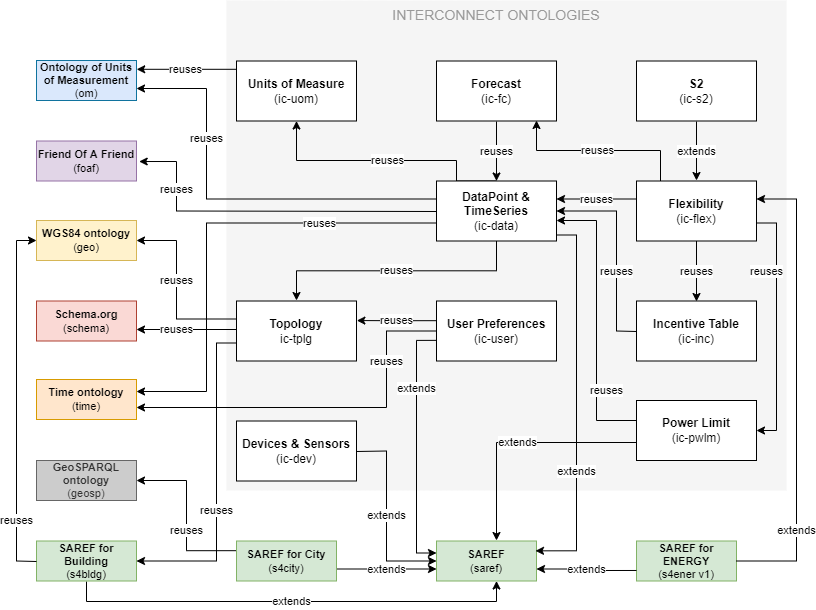
\includegraphics[width=\textwidth]{figures/panoramicaInterconnect.png}
    \caption{Panoramica delle ontologie InterConnect in relazione a SAREF e ad altre ontologie esistenti.}
    \label{fig:panoramicaInterconnect}
\end{figure}

\subsection{Ontologie create nel progetto Interconnect}
Nel progetto Interconnect sono state sviluppate nove ontologie. Vengono presentate nella tabella \ref{tab:ontologieCreate}
\begin{table}[H]
    \centering
    \begin{tabularx}{\textwidth}{|X|X|X|}
        \hline
        Prefisso & Namespace                                                         & Concetti                                                                                            \\
        \hline
        ic-data  & \href{http://ontology.tno.nl/interconnect/datapoint\#}{link}      & Datapoint, TimeSeries, Message, Utility Purpose                                                     \\
        ic-dev   & \href{http://ontology.tno.nl/interconnect/device\#}{link}         & Device, State, Function                                                                             \\
        ic-flex  & \href{http://ontology.tno.nl/interconnect/flexibility\#}{link}    & Flex Offer, Flexibility Source, Control Type, Power Envelope                                        \\
        ic-fc    & \href{http://ontology.tno.nl/interconnect/forecast\#}{link}       & Forecast, Point Forecast, Stochastic Forecast (Gaussian, Quantile, Trajectory), Gaussian Data Point \\
        ic-inc   & \href{http://ontology.tno.nl/interconnect/incentivetable\#}{link} & Incentive Table, Incentive Tiers, Scope and Type                                                    \\
        ic-pwlm  & \href{http://ontology.tno.nl/interconnect/powerlimit\#}{link}     & Power Limit (Nominal, Contractual and Failsafe)                                                     \\
        ic-tplg  & \href{http://ontology.tno.nl/interconnect/topology\#}{link}       & Topological Location, Grid Segment, Market Segment, Regulation Zone, Electrical Phases              \\
        ic-uom   & \href{http://ontology.tno.nl/interconnect/units\#}{link}          & Additional Units of Measure (not considered yet in SAREF)                                           \\
        ic-user  & \href{http://ontology.tno.nl/interconnect/user\#}{link}           & User, User Profile, Preference, Priority, Interest, Activity, Time, Location                        \\
        \hline
    \end{tabularx}
    \caption{Ontologie create all'interno del progetto Interconnect}
    \label{tab:ontologieCreate}
\end{table}

\subsection{Ontologie utilizzate}
L'utilizzo di altre ontologie è uno dei pilastri del web semantico. Nella tabella \ref{tab:ontologieUtilizzate} vengono elencate tutte le ontologie utilizzate nel progetto Interconnect, con relativo dettaglio sui concetti di tali librerie.
\begin{table}[H]
    \centering
    \begin{tabularx}{\textwidth}{|X|X|X|}
        \hline
        Prefisso & Namespace                                                               & Concetti                                                                            \\
        \hline
        foaf     & \href{http://xmlns.com/foaf/0.1/}{link}                                 & Agent                                                                               \\
        geo      & \href{http://www.w3.org/2003/01/geo/wgs84_pos}{link}                    & Spatial Thing, geo coordinates                                                      \\
        geosp    & \href{http://www.opengis.net/ont/geosparql}{link}                       & Geographical Feature                                                                \\
        schema   & \href{https://schema.org/}{link}                                        & Address, Countries, Postal Codes                                                    \\
        om       & \href{http://www.ontology-of-units-of-measure.org/resource/om-2/}{link} & Quantity, Unit, Measure                                                             \\
        saref    & \href{https://saref.etsi.org/core/}{link}                               & Device, Function, Command, State, Measurement, Unit of Measure, Feature of Interest \\
        s4bldg   & \href{https://saref.etsi.org/saref4bldg/}{link}                         & Building, Building Space, Building Object                                           \\
        s4city   & \href{https://saref.etsi.org/saref4ener/}{link}                         & Power Profile, Alternatives, Power Sequence, Slot                                   \\
        s4ener   & \href{https://saref.etsi.org/saref4city/}{link}                         & Facility, Administrative Area, City Object                                          \\
        time     & \href{http://www.w3.org/2006/time}{link}                                & Instant, Interval, Duration                                                         \\
        \hline
    \end{tabularx}
    \caption{Ontologie utilizzate all'interno del progetto Interconnect}
    \label{tab:ontologieUtilizzate}
\end{table}

\section{InterConnect Interoperability Framework}
La parte interessante di questo progetto è l'Interoperability Framework che viene fornito.
Questo Interoperability Framework è capace di colmare le lacune di interoperabilità all'interno e tra i domini dell'energia e dell'IoT.

\begin{figure}[H]
    \centering
    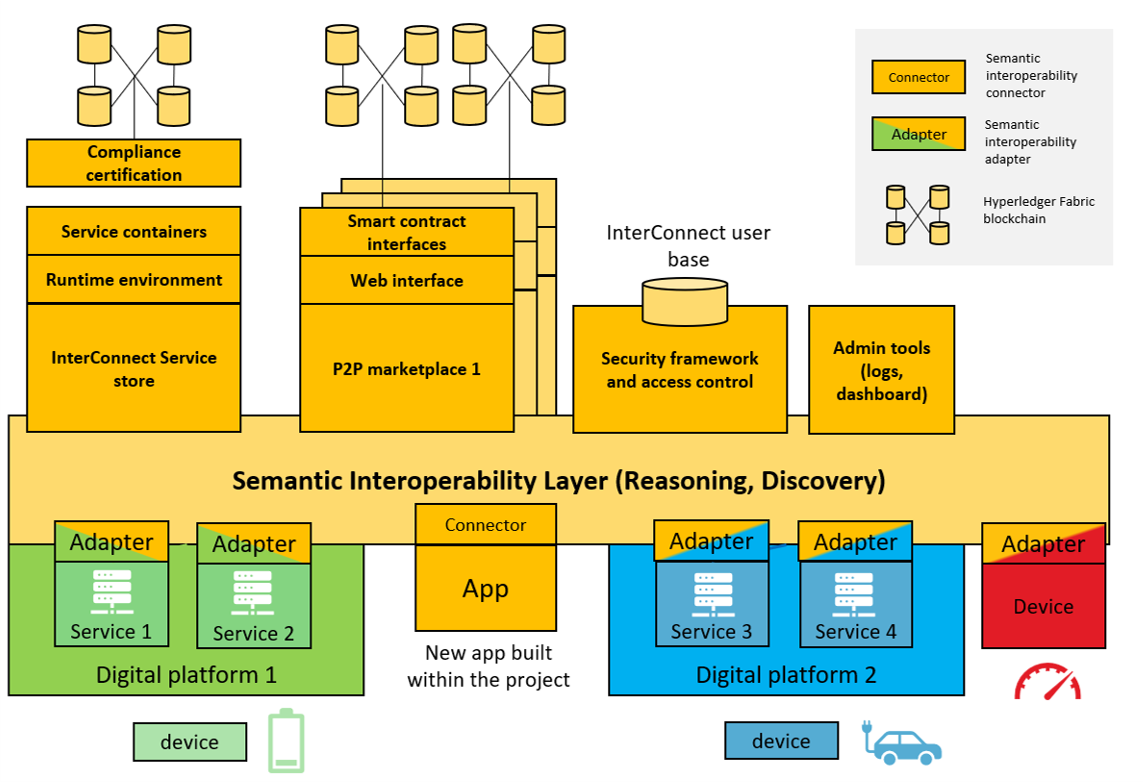
\includegraphics[width=\textwidth]{figures/architetturaFrameworkInterconnect.png}
    \caption{Architettura di alto livello dell'InterConnect Interoperability Framework.}
    \label{fig:architetturaFrameworkInterconnect}
\end{figure}

Di seguito vengono elencati i tre componenti principali del Framework:
\begin{itemize}
    \item InterConnect Service Store;
    \item Semantic Interoperability Layer;
    \item P2P MarketPlace.
\end{itemize}

\paragraph{InterConnect Service Store}

Il Service Store non è altro che un'applicazione web dove è necessario registrarsi per poter utilizzare e fornire servizi in maniera interoperabile. Riguarda sia servizi provenienti da settori energetici sia servizi che non riguardano il dominio dell'energia.
È possibile accedere al Service Store dal seguente \href{https://store.interconnectproject.eu/ServiceStore}{link: Service Store}.

L'obiettivo principale è quello di favorire lo sviluppo dell'ecosistema InterConnect, in cui fornitori e utilizzatori di servizi possano collaborare in modo più efficace. Questo sarà possibile grazie alla possibilità di registrare nuovi servizi interoperabili e di consultare quelli già esistenti, al fine di individuare quelli più adatti alle proprie esigenze e di ottenere tutte le informazioni necessarie per accedere e utilizzare correttamente i servizi selezionati. In questo modo, si creerà un punto di riferimento unico per tutti gli utenti dell'ecosistema InterConnect, con benefici in termini di semplificazione dell'accesso alle informazioni e miglioramento della qualità dei servizi offerti.


\paragraph{Semantic Interoperability Layer (SIL)}
Il Semantic Interoperability Layer è il componente principale del framework. È responsabile dello scambio di conoscenza tra tutti i componenti e servizi interoperabili.
Il SIL è composto da più moduli, elencati di seguito:
\begin{itemize}
    \item knowledge engine: è il componente che gestisce la conoscenza semantica all'interno del sistema. Questo modulo si occupa di archiviare, gestire e interrogare le ontologie, i dati semantici e le regole di inferenza del sistema;
    \item Generic adapter: il suo compito principale è di mediare l'interazione tra le applicazioni e il sistema InterConnect, convertendo i dati tra i formati dei diversi sistemi e garantendo l'interoperabilità semantica tra di essi;
    \item Ontologie: vanno usate ontologie già esistenti (ad esempio SAREF) per definire uno standard per il dominio;
    \item Reasoning: si occupa di inferire nuove informazioni dai dati esistenti all'interno del sistema InterConnect;
    \item Discovery: consente la scoperta di servizi e risorse all'interno del sistema InterConnect, migliorando così la collaborazione e lo scambio di informazioni tra organizzazioni diverse.
\end{itemize}

Oltre ai moduli principali di cui abbiamo parlato, il Semantic Interoperability Layer di InterConnect include anche altri strumenti che possono supportare la creazione e la gestione di un sistema interoperabile:
\begin{itemize}
    \item SSA Test Tool: permette di verificare se i servizi semantici implementati seguono correttamente gli standard e le best practice definiti dall'architettura SSA. Lo strumento permette di eseguire test di interoperabilità, di conformità ai requisiti e di performance sui servizi semantici, generando report dettagliati sull'esito dei test;
    \item Graph Pattern Visualizer: strumento che consente di visualizzare graficamente i graph pattern. Grazie alla rappresentazione visuale, è possibile verificare loop o altre inconsistenze tra soggetti, predicati e oggetti del grafo;
    \item Graph Pattern Syntax Checker: strumento che permette l'individuazione degli errori di sintassi nei graph pattern, in modo rapido ed efficiente.
\end{itemize}



\paragraph{P2P MarketPlace}
Il P2P MarketPlace di InterConnect si basa sul progetto blockchain open source Hyperledger e permette la creazione di casi d'uso decentralizzati pur continuando a utilizzare l'InterConnect Interoperability Framework.


\chapter{Ontologie per Energy Storage System}

L'obiettivo principale delle ontologie per \textit{Energy Storage System} (ESS)
è di fornire una descrizione
semantica standardizzata dei dati relativi agli ESS, in modo da consentire
l'interoperabilità tra i sistemi di gestione dell'energia e i dispositivi ESS
provenienti da diversi fornitori. Questa interoperabilità è essenziale per
garantire l'efficienza, l'affidabilità e la sicurezza delle reti elettriche
intelligenti (smart grid) e per consentire l'integrazione di fonti di energia
rinnovabile.

Le ontologie ESS comprendono concetti come la capacità di stoccaggio
dell'energia, la capacità di erogazione di potenza, la capacità di ricarica, il
livello di sicurezza e
molti altri. Questi concetti sono organizzati in una struttura gerarchica che
definisce le relazioni tra di essi.

Esistono molte ontologie che coprono questi aspetti e ne estendono i concetti,
tra cui: \textit{OntoPowSys}, \textit{Energy Storage Systems Ontology},
\textit{Open Energy Ontology} e l'ecosistema basato su \textit{EMMO}.

\section{OntoPowSys}
OntoPowSys \cite{OntoPowSys} è un'ontologia del dominio dei sistemi di
alimentazione, che è stata
sviluppata con lo scopo di supportare l'analisi e la progettazione di sistemi
di alimentazione elettrica, in particolare per applicazioni industriali e di
produzione di energia rinnovabile.

Si basa su una struttura a tre livelli, che comprende:
la descrizione dei componenti, la descrizione delle funzioni e la descrizione
delle proprietà.

L'ontologia è stata utilizzata per sviluppare strumenti di supporto alla
decisione per l'analisi e la progettazione dei sistemi di alimentazione
elettrica, ad esempio per la selezione e la configurazione dei componenti del
sistema. Inoltre, OntoPowSys è stato integrato con altre ontologie del dominio
dell'energia, come la Open Energy Ontology, per creare una visione più completa
e integrata del sistema energetico.

Oltre a questo OntoPowSys estende i concetti di supporto creando un framework per l'esecuzione
di modelli matematici in JPS (Joint Processing System è un sistema informatico
che
utilizza ontologie per integrare conoscenze provenienti da diverse fonti e
consentire l'esecuzione di studi e simulazioni).

\subsection{Casi d'uso}
In seguito verrà presentato qualche esempio di applicazione dell'ontologia
OntoPowSys.

\subsubsection{Optimal Power Flow}
OntoPowSys è stata integrata nell'agente Optimal Power Flow (OPF) della
piattaforma JPS, che consente di risolvere il problema dell'ottimizzazione
della distribuzione di energia elettrica. Esso utilizza l'ontologia
OntoPowSys per acquisire conoscenze sul sistema elettrico e fornire soluzioni
ottimali al problema dell'OPF.

Le informazioni vengono acquisite tramite query
SPARQL sul grafo di conoscenza JPS e utilizzate per eseguire i modelli
matematici. I risultati vengono aggiornati nel grafo di conoscenza e
visualizzati tramite strumenti appositi.

\subsubsection{Bio Diesel Plant Simulation}
Nell'ambito della simulazione di una bio-raffineria, OntoPowSys viene
utilizzata per la modellizzazione delle proprietà dei materiali coinvolti nei
processi di produzione del biodiesel. Questi modelli vengono integrati nella
piattaforma JPS, che utilizza web services e agenti specifici per eseguire
simulazioni e analisi.

In particolare, un agente di JPS viene utilizzato per lo
studio delle interazioni tra le varie fasi del processo di produzione del
biodiesel. Le informazioni raccolte dalla simulazione vengono utilizzate per
aggiornare la conoscenza presente nella piattaforma JPS e per generare
risultati visualizzabili tramite appositi strumenti.

\section{Open Energy Ontology}
Open Energy Ontology \cite{OpenEnergyOntology} (OEO) è un'ontologia di dominio
nel campo della
modellizzazione dei sistemi energetici. Ha lo scopo di standardizzare la
terminologia nel campo e di fornire una struttura logica per l'integrazione dei
dati e l'aggregazione. L'ontologia può essere utilizzata anche per la creazione
di modelli di acquisizione dei dati, la visualizzazione dei dati e l'estrazione
di informazioni dal testo e dai dati.

Gli obiettivi dell'Open Energy Ontology \cite{OEO} sono orientati alla
crescente
sofisticazione e interdipendenza della modellizzazione dei sistemi energetici.
Ciò richiede una maggiore automazione delle interfacce tra modelli e una
comprensione semantica dei dati.

\subsection{Casi d'uso}
In seguito verranno descritti casi d'uso provenienti dai progetti
\textit{SzenarienDB}, \textit{LOD-GEOSS} e \textit{SIROP}.

\subsubsection{Scenario description}
Lo scopo era quello di creare un quadro che permettesse di collegare in modo
più strutturato e trasparente i risultati di ricerche energetiche, le basi di
dati utilizzate e le assunzioni implicite ed esplicite coinvolte.

Da una raccolta di proprietà degli scenari e degli
studi energetici che coprono le informazioni più importanti, proprietà inserite
in un foglio di calcolo da cui è stato creato un
grafo di conoscenza RDF, che utilizza
le classi e le relazioni definite nella OEO sulla base di questi fogli di
calcolo.

La piattaforma Open Energy è stata estesa con una sezione aggiuntiva che
consente agli utenti
di visualizzare ed editare le informazioni memorizzate nel grafo di conoscenza.
Questo permette ai ricercatori di rendere la loro ricerca più disponibile al
pubblico e facilita una descrizione più strutturata del paesaggio di basi di
dati, modelli energetici e risultati scientifici.

\subsubsection{Data representation for the core energy market data register}
Il registro centrale dei dati del mercato energetico (MaStR) pubblicato
dall'Agenzia federale tedesca per le reti energetiche nel 2019 fornisce una
lista completa di tutte le centrali registrate in Germania che si connettono
alla rete. Tuttavia, l'API del MaStR è complessa e presenta limitazioni
nell'accesso ai dati, come ad esempio il numero limitato di richieste
giornaliere per utente.

Per migliorare l'accessibilità ai dati, è stato
sviluppato uno strumento open source per estrarre dati dal MaStR, arricchendoli
con metadati e rendendoli disponibili sulla piattaforma Open Energy Platform,
dove possono essere scaricati senza bisogno di registrazione.

Con l'Ontology
for Energy Systems (OEO) è possibile annotare il dataset MaStR e semplificare
le query complesse attraverso una mappatura dell'API a un endpoint per il
protocollo SPARQL che utilizza i termini definiti nell'ontologia. Ciò permette
una maggiore facilità d'uso per la raccolta di dati complessi e l'arricchimento
del dataset con dipendenze logiche.

\subsubsection{Data annotation of an energy meteorological time series data
      set}

Questo caso d'uso tratta dell'annotazione di serie temporali meteorologiche
energetiche utilizzate come
dati di input o output in modelli di sistemi energetici. L'annotazione coerente
e completa non è banale poiché esistono diverse modalità
di descrizione delle serie temporali e le convenzioni di annotazione variano a
seconda dei domini.

L'OEO facilita questo processo fornendo definizioni concise e non ambigue per i
diversi concetti di annotazione. Ciò consente alla struttura e al contenuto
delle serie temporali meteorologiche energetiche e di altre discipline di
essere descritte completamente e identificate senza sforzo interdisciplinare.

\subsubsection{Interface homogenization of the FINE energy system model
      framework}

Utilizzando l'OEO, si vuole omogeneizzare l'annotazione all'interno di un
database distribuito di inventari di dati e parametri funzionali attesi o
forniti dalle interfacce dei modelli.
Si riduce l'eterogeneità delle descrizioni delle interfacce e si minimizza lo
sforzo dei programmatori e
degli utenti per produrle e comprenderle.

Sulla base della descrizione dell'interfaccia attualmente esistente in cui i
singoli parametri di funzione sono denominati e definiti, si sta attualmente
esplorando in che misura esiste già una copertura con la terminologia dell'OEO
e in che punti è necessario adattare l'interfaccia o l'ontologia. Utilizzando
queste applicazioni specifiche del modello, si mira a sviluppare le migliori
pratiche che possono essere utilizzate per omogeneizzare la connessione dei
dati ai modelli e, alla fine, lo scambio di dati tra i modelli stessi e per
promuovere lo scambio scientifico all'interno della comunità internazionale del
sistema energetico.

\section{Energy Storage Systems Ontology}
L'Energy Storage Systems Ontology \cite{EnergyStorageSystemOntology} è
un'ontologia, che dispone di 10 classi, sviluppata per
rappresentare le conoscenze e le informazioni relative ai sistemi di accumulo
dell'energia (ESS). Questa ontologia è un modulo del “Domain Analysis-Based
Global Energy ontology” e si occupa di rappresentare dispositivi di accumulo di
energia, come batterie o condensatori.

\section{EMMO-based Ecosystem}
Elementary Multiperspective Material Ontology (EMMO) \cite{emmo} è un
framework ontologico per le
scienze applicate e l'ingegneria. È stato progettato per soddisfare le esigenze
di una descrizione semantica profondamente radicata nelle scienze fisiche,
incorporando la descrizione dei materiali da una rigorosa prospettiva fisica,
le relazioni formali tra livelli di granularità per facilitare la descrizione
di materiali multi-scala e la definizione di processi materiali per catturare
il cambiamento ed evoluzione dei materiali come catena di diversi stati.

Attualmente definisce quattro prospettive:
\begin{itemize}
      \item \textbf{Riduzionistica}: introduce una relazione di
            parzialità diretta non transitiva.
      \item \textbf{Fisicalistica}: categorizza il mondo
            secondo la fisica applicata.
      \item \textbf{Percettuale}: categorizza gli oggetti del mondo reale in base
            a come sono percepiti dall'utente come modello riconoscibile nello
            spazio o nel tempo.
      \item \textbf{Olistica}: si occupa dei processi che si svolgono nel tempo e
            del ruolo dei diversi partecipanti al processo. Uno di questi
            processi è
            chiamato semiosi. In una semiosi un interprete collega un oggetto ad
            un segno
            che gli dà significato.
\end{itemize}

Lo sviluppo e l'uso di EMMO è supportato dal Consiglio europeo per la
modellizzazione dei materiali (EMMC), che mira ad avvicinare la modellizzazione
dei materiali alle esigenze dell'industria. Uno dei principali obiettivi
dell'EMMC è di facilitare l'interoperabilità dei dati e dei modelli tra diversi
domini tecnici. Questo viene fatto attraverso l'istituzione di schemi di
metadati comuni e roadmap, che possono essere utilizzati come guida per le
ontologie di dominio EMMO.

\subsection{Caso d'uso}

\subsubsection{BattINFO}
BattINFO \cite{emmo} è un'ontologia di dominio per le celle batteria, i
componenti, i materiali e le loro interfacce, sviluppata per supportare
l'interoperabilità dei dati e i flussi di lavoro di intelligenza artificiale.
BattINFO si basa sull'ontologia EMMO e include un'ontologia di elettrochimica
come base fondamentale. Le classi di quest'ontologia si basano sulle
raccomandazioni
dell'International Union of Pure and Applied Chemistry (IUPAC) e della
International Electrotechnical Commission (IEC). L'ontologia fornisce anche
annotazioni per definire le etichette preferite per l'entità "Battery", oltre a
collegamenti alle voci di Wikipedia e dbpedia.

\section{Problematiche}
La problematica principale dell'esistenza di tutte queste ontologie è che non
sono correlate le une con le altre.

Le ontologie sopra elencate non sono allineate con SAREF, ciò comporta la
limitazione della riusabilità all'interno delle iniziative basate su SAREF e
viceversa.

Sarebbe consono a riguardo scegliere di adottare uno standard comune a tutti i
progetti inerenti a questi ambiti, in maniera tale da favorirne la comprensione
e il riutilizzo, nonchè la manutenibilità nel tempo.

\bibliography{bibliography}
\bibliographystyle{plain}

\end{document}